% Options for packages loaded elsewhere
\PassOptionsToPackage{unicode}{hyperref}
\PassOptionsToPackage{hyphens}{url}
%
\documentclass[
]{article}
\usepackage{lmodern}
\usepackage{amssymb,amsmath}
\usepackage{ifxetex,ifluatex}
\ifnum 0\ifxetex 1\fi\ifluatex 1\fi=0 % if pdftex
  \usepackage[T1]{fontenc}
  \usepackage[utf8]{inputenc}
  \usepackage{textcomp} % provide euro and other symbols
\else % if luatex or xetex
  \usepackage{unicode-math}
  \defaultfontfeatures{Scale=MatchLowercase}
  \defaultfontfeatures[\rmfamily]{Ligatures=TeX,Scale=1}
\fi
% Use upquote if available, for straight quotes in verbatim environments
\IfFileExists{upquote.sty}{\usepackage{upquote}}{}
\IfFileExists{microtype.sty}{% use microtype if available
  \usepackage[]{microtype}
  \UseMicrotypeSet[protrusion]{basicmath} % disable protrusion for tt fonts
}{}
\makeatletter
\@ifundefined{KOMAClassName}{% if non-KOMA class
  \IfFileExists{parskip.sty}{%
    \usepackage{parskip}
  }{% else
    \setlength{\parindent}{0pt}
    \setlength{\parskip}{6pt plus 2pt minus 1pt}}
}{% if KOMA class
  \KOMAoptions{parskip=half}}
\makeatother
\usepackage{xcolor}
\IfFileExists{xurl.sty}{\usepackage{xurl}}{} % add URL line breaks if available
\IfFileExists{bookmark.sty}{\usepackage{bookmark}}{\usepackage{hyperref}}
\hypersetup{
  pdftitle={Problem Set 1},
  pdfauthor={Answer Key},
  hidelinks,
  pdfcreator={LaTeX via pandoc}}
\urlstyle{same} % disable monospaced font for URLs
\usepackage[margin=1in]{geometry}
\usepackage{color}
\usepackage{fancyvrb}
\newcommand{\VerbBar}{|}
\newcommand{\VERB}{\Verb[commandchars=\\\{\}]}
\DefineVerbatimEnvironment{Highlighting}{Verbatim}{commandchars=\\\{\}}
% Add ',fontsize=\small' for more characters per line
\usepackage{framed}
\definecolor{shadecolor}{RGB}{248,248,248}
\newenvironment{Shaded}{\begin{snugshade}}{\end{snugshade}}
\newcommand{\AlertTok}[1]{\textcolor[rgb]{0.94,0.16,0.16}{#1}}
\newcommand{\AnnotationTok}[1]{\textcolor[rgb]{0.56,0.35,0.01}{\textbf{\textit{#1}}}}
\newcommand{\AttributeTok}[1]{\textcolor[rgb]{0.77,0.63,0.00}{#1}}
\newcommand{\BaseNTok}[1]{\textcolor[rgb]{0.00,0.00,0.81}{#1}}
\newcommand{\BuiltInTok}[1]{#1}
\newcommand{\CharTok}[1]{\textcolor[rgb]{0.31,0.60,0.02}{#1}}
\newcommand{\CommentTok}[1]{\textcolor[rgb]{0.56,0.35,0.01}{\textit{#1}}}
\newcommand{\CommentVarTok}[1]{\textcolor[rgb]{0.56,0.35,0.01}{\textbf{\textit{#1}}}}
\newcommand{\ConstantTok}[1]{\textcolor[rgb]{0.00,0.00,0.00}{#1}}
\newcommand{\ControlFlowTok}[1]{\textcolor[rgb]{0.13,0.29,0.53}{\textbf{#1}}}
\newcommand{\DataTypeTok}[1]{\textcolor[rgb]{0.13,0.29,0.53}{#1}}
\newcommand{\DecValTok}[1]{\textcolor[rgb]{0.00,0.00,0.81}{#1}}
\newcommand{\DocumentationTok}[1]{\textcolor[rgb]{0.56,0.35,0.01}{\textbf{\textit{#1}}}}
\newcommand{\ErrorTok}[1]{\textcolor[rgb]{0.64,0.00,0.00}{\textbf{#1}}}
\newcommand{\ExtensionTok}[1]{#1}
\newcommand{\FloatTok}[1]{\textcolor[rgb]{0.00,0.00,0.81}{#1}}
\newcommand{\FunctionTok}[1]{\textcolor[rgb]{0.00,0.00,0.00}{#1}}
\newcommand{\ImportTok}[1]{#1}
\newcommand{\InformationTok}[1]{\textcolor[rgb]{0.56,0.35,0.01}{\textbf{\textit{#1}}}}
\newcommand{\KeywordTok}[1]{\textcolor[rgb]{0.13,0.29,0.53}{\textbf{#1}}}
\newcommand{\NormalTok}[1]{#1}
\newcommand{\OperatorTok}[1]{\textcolor[rgb]{0.81,0.36,0.00}{\textbf{#1}}}
\newcommand{\OtherTok}[1]{\textcolor[rgb]{0.56,0.35,0.01}{#1}}
\newcommand{\PreprocessorTok}[1]{\textcolor[rgb]{0.56,0.35,0.01}{\textit{#1}}}
\newcommand{\RegionMarkerTok}[1]{#1}
\newcommand{\SpecialCharTok}[1]{\textcolor[rgb]{0.00,0.00,0.00}{#1}}
\newcommand{\SpecialStringTok}[1]{\textcolor[rgb]{0.31,0.60,0.02}{#1}}
\newcommand{\StringTok}[1]{\textcolor[rgb]{0.31,0.60,0.02}{#1}}
\newcommand{\VariableTok}[1]{\textcolor[rgb]{0.00,0.00,0.00}{#1}}
\newcommand{\VerbatimStringTok}[1]{\textcolor[rgb]{0.31,0.60,0.02}{#1}}
\newcommand{\WarningTok}[1]{\textcolor[rgb]{0.56,0.35,0.01}{\textbf{\textit{#1}}}}
\usepackage{graphicx,grffile}
\makeatletter
\def\maxwidth{\ifdim\Gin@nat@width>\linewidth\linewidth\else\Gin@nat@width\fi}
\def\maxheight{\ifdim\Gin@nat@height>\textheight\textheight\else\Gin@nat@height\fi}
\makeatother
% Scale images if necessary, so that they will not overflow the page
% margins by default, and it is still possible to overwrite the defaults
% using explicit options in \includegraphics[width, height, ...]{}
\setkeys{Gin}{width=\maxwidth,height=\maxheight,keepaspectratio}
% Set default figure placement to htbp
\makeatletter
\def\fps@figure{htbp}
\makeatother
\setlength{\emergencystretch}{3em} % prevent overfull lines
\providecommand{\tightlist}{%
  \setlength{\itemsep}{0pt}\setlength{\parskip}{0pt}}
\setcounter{secnumdepth}{-\maxdimen} % remove section numbering

\title{Problem Set 1}
\author{Answer Key}
\date{ECON 480 --- Fall 2020}

\begin{document}
\maketitle

Answers may be longer than I would deem sufficient on an exam. Some
might vary slightly based on points of interest, examples, or personal
experience. These suggested answers are designed to give you both the
answer and a short explanation of \emph{why} it is the answer.

\hypertarget{the-popularity-of-baby-names}{%
\section{The Popularity of Baby
Names}\label{the-popularity-of-baby-names}}

\textbf{Install and load the package \texttt{babynames}. Get help for
\texttt{?babynames} to see what the data includes.}

\begin{Shaded}
\begin{Highlighting}[]
\KeywordTok{library}\NormalTok{(tidyverse)}
\end{Highlighting}
\end{Shaded}

\begin{verbatim}
## -- Attaching packages ------------------------------------------------------------------------------------ tidyverse 1.3.0 --
\end{verbatim}

\begin{verbatim}
## v ggplot2 3.3.2     v purrr   0.3.4
## v tibble  3.0.3     v dplyr   1.0.2
## v tidyr   1.1.1     v stringr 1.4.0
## v readr   1.3.1     v forcats 0.5.0
\end{verbatim}

\begin{verbatim}
## -- Conflicts --------------------------------------------------------------------------------------- tidyverse_conflicts() --
## x dplyr::filter() masks stats::filter()
## x dplyr::lag()    masks stats::lag()
\end{verbatim}

\begin{Shaded}
\begin{Highlighting}[]
\CommentTok{# install for first use}
\CommentTok{# install.packages("babynames")}

\CommentTok{# load package }
\KeywordTok{library}\NormalTok{(babynames)}

\CommentTok{# explore help}
\CommentTok{# ?babynames}
\end{Highlighting}
\end{Shaded}

\hypertarget{question-1}{%
\subsection{Question 1}\label{question-1}}

\hypertarget{part-a}{%
\subsubsection{Part A}\label{part-a}}

\textbf{What are the top 5 boys names for 2017, and what \emph{percent}
of overall names is each?}

\begin{Shaded}
\begin{Highlighting}[]
\CommentTok{# save as a new tibble}
\NormalTok{top_}\DecValTok{5}\NormalTok{_boys_}\DecValTok{2017}\NormalTok{ <-}\StringTok{ }\NormalTok{babynames }\OperatorTok\StringTok{ }\CommentTok{# take data}
\StringTok{  }\KeywordTok{filter}\NormalTok{(sex}\OperatorTok{==}\StringTok{"M"}\NormalTok{, }\CommentTok{# filter by males}
\NormalTok{         year}\OperatorTok{==}\DecValTok{2017}\NormalTok{) }\OperatorTok\StringTok{ }\CommentTok{# and for 2007}
\StringTok{  }\KeywordTok{arrange}\NormalTok{(}\KeywordTok{desc}\NormalTok{(n)) }\OperatorTok\StringTok{ }\CommentTok{# arrange in largest-to-smallest order of n (number)}
\StringTok{  }\KeywordTok{slice}\NormalTok{(}\DecValTok{1}\OperatorTok{:}\DecValTok{5}\NormalTok{) }\OperatorTok\StringTok{ }\CommentTok{# optional, look only at first 5 rows; head(., n=5) also works}
\StringTok{  }\KeywordTok{mutate}\NormalTok{(}\DataTypeTok{percent =} \KeywordTok{round}\NormalTok{(prop}\OperatorTok{*}\DecValTok{100}\NormalTok{, }\DecValTok{2}\NormalTok{)) }\CommentTok{# also optional, make a percent variable rounded to 2 decimals}

\CommentTok{# look at our new tibble}
\NormalTok{top_}\DecValTok{5}\NormalTok{_boys_}\DecValTok{2017}
\end{Highlighting}
\end{Shaded}

\begin{verbatim}
## # A tibble: 5 x 6
##    year sex   name        n    prop percent
##   <dbl> <chr> <chr>   <int>   <dbl>   <dbl>
## 1  2017 M     Liam    18728 0.00954    0.95
## 2  2017 M     Noah    18326 0.00933    0.93
## 3  2017 M     William 14904 0.00759    0.76
## 4  2017 M     James   14232 0.00725    0.72
## 5  2017 M     Logan   13974 0.00712    0.71
\end{verbatim}

The top 5 names are

\begin{enumerate}
\def\labelenumi{\arabic{enumi}.}
\tightlist
\item
  Liam (0.95\%)
\item
  Noah (0.93\%)
\item
  William (0.76\%)
\item
  James (0.72\%)
\item
  Logan (0.71\%)
\end{enumerate}

\hypertarget{part-b}{%
\subsubsection{Part B}\label{part-b}}

\textbf{What are the top 5 \emph{girls} names, and what \emph{percent}
of overall names is each?}

\begin{Shaded}
\begin{Highlighting}[]
\CommentTok{# save as a new tibble}
\NormalTok{top_}\DecValTok{5}\NormalTok{_girls_}\DecValTok{2017}\NormalTok{ <-}\StringTok{ }\NormalTok{babynames }\OperatorTok\StringTok{ }\CommentTok{# take data}
\StringTok{  }\KeywordTok{filter}\NormalTok{(sex}\OperatorTok{==}\StringTok{"F"}\NormalTok{, }\CommentTok{# filter by females}
\NormalTok{         year}\OperatorTok{==}\DecValTok{2017}\NormalTok{) }\OperatorTok\StringTok{ }\CommentTok{# and for 2007}
\StringTok{  }\KeywordTok{arrange}\NormalTok{(}\KeywordTok{desc}\NormalTok{(n)) }\OperatorTok\StringTok{ }\CommentTok{# arrange in largest-to-smallest order of n (number)}
\StringTok{  }\KeywordTok{slice}\NormalTok{(}\DecValTok{1}\OperatorTok{:}\DecValTok{5}\NormalTok{) }\OperatorTok\StringTok{ }\CommentTok{# optional, look only at first 5 rows; head(., n=5) also works}
\StringTok{  }\KeywordTok{mutate}\NormalTok{(}\DataTypeTok{percent =} \KeywordTok{round}\NormalTok{(prop}\OperatorTok{*}\DecValTok{100}\NormalTok{, }\DecValTok{2}\NormalTok{)) }\CommentTok{# also optional, make a percent variable rounded to 2 decimals}

\CommentTok{# look at our new tibble}
\NormalTok{top_}\DecValTok{5}\NormalTok{_girls_}\DecValTok{2017}
\end{Highlighting}
\end{Shaded}

\begin{verbatim}
## # A tibble: 5 x 6
##    year sex   name         n    prop percent
##   <dbl> <chr> <chr>    <int>   <dbl>   <dbl>
## 1  2017 F     Emma     19738 0.0105     1.05
## 2  2017 F     Olivia   18632 0.00994    0.99
## 3  2017 F     Ava      15902 0.00848    0.85
## 4  2017 F     Isabella 15100 0.00805    0.81
## 5  2017 F     Sophia   14831 0.00791    0.79
\end{verbatim}

The top 5 names are

\begin{enumerate}
\def\labelenumi{\arabic{enumi}.}
\tightlist
\item
  Emma (1.05\%)
\item
  Olivia (0.99\%)
\item
  Ava (0.85\%)
\item
  Isabella (0.81\%)
\item
  Sophia (0.79\%)
\end{enumerate}

\hypertarget{question-2}{%
\subsection{Question 2}\label{question-2}}

\textbf{Make two barplots, of these top 5 names, one for each sex. Map
\texttt{aes}thetics \texttt{x} to \texttt{name} and \texttt{y} to
\texttt{prop}\footnote{Or \texttt{percent}, if you made that variable,
  as I did.} and use \texttt{geom\_col} (since you are declaring a
specific \texttt{y}, otherwise you could just use \texttt{geom\_bar()}
and just an \texttt{x}.)}

\begin{Shaded}
\begin{Highlighting}[]
\KeywordTok{ggplot}\NormalTok{(}\DataTypeTok{data =}\NormalTok{ top_}\DecValTok{5}\NormalTok{_boys_}\DecValTok{2017}\NormalTok{)}\OperatorTok{+}
\StringTok{  }\KeywordTok{aes}\NormalTok{(}\DataTypeTok{x =} \KeywordTok{reorder}\NormalTok{(name, n), }\CommentTok{#note this reorders the x variable from small to large n}
      \DataTypeTok{y =}\NormalTok{ percent, }\CommentTok{# you can use prop if you didn't make a percent variable}
      \DataTypeTok{fill =}\NormalTok{ name)}\OperatorTok{+}\StringTok{ }\CommentTok{# optional color!}
\StringTok{  }\KeywordTok{geom_col}\NormalTok{()}\OperatorTok{+}
\StringTok{  }
\StringTok{  }\CommentTok{# now I'm just making it pretty}
\StringTok{  }\KeywordTok{scale_y_continuous}\NormalTok{(}\DataTypeTok{labels=}\ControlFlowTok{function}\NormalTok{(x)}\KeywordTok{paste}\NormalTok{(x,}\StringTok{"%"}\NormalTok{,}\DataTypeTok{sep=}\StringTok{""}\NormalTok{))}\OperatorTok{+}\StringTok{ }\CommentTok{# optional, add percent signs}
\StringTok{      }\KeywordTok{labs}\NormalTok{(}\DataTypeTok{x =} \StringTok{"Name"}\NormalTok{,}
         \DataTypeTok{y =} \StringTok{"Percent of All Babies With Name"}\NormalTok{,}
         \DataTypeTok{title =} \StringTok{"Most Popular Boys Names Since 1880"}\NormalTok{,}
         \DataTypeTok{fill =} \StringTok{"Boy's Name"}\NormalTok{,}
         \DataTypeTok{caption =} \StringTok{"Source: SSA"}\NormalTok{)}\OperatorTok{+}
\StringTok{    }\KeywordTok{theme_classic}\NormalTok{(}\DataTypeTok{base_family =} \StringTok{"Fira Sans Condensed"}\NormalTok{, }\DataTypeTok{base_size=}\DecValTok{16}\NormalTok{)}\OperatorTok{+}
\StringTok{  }\KeywordTok{coord_flip}\NormalTok{()}\OperatorTok{+}\StringTok{ }\CommentTok{# rotate axes!}
\StringTok{  }\KeywordTok{theme}\NormalTok{(}\DataTypeTok{legend.position =} \StringTok{""}\NormalTok{) }\CommentTok{# hide legend}
\end{Highlighting}
\end{Shaded}

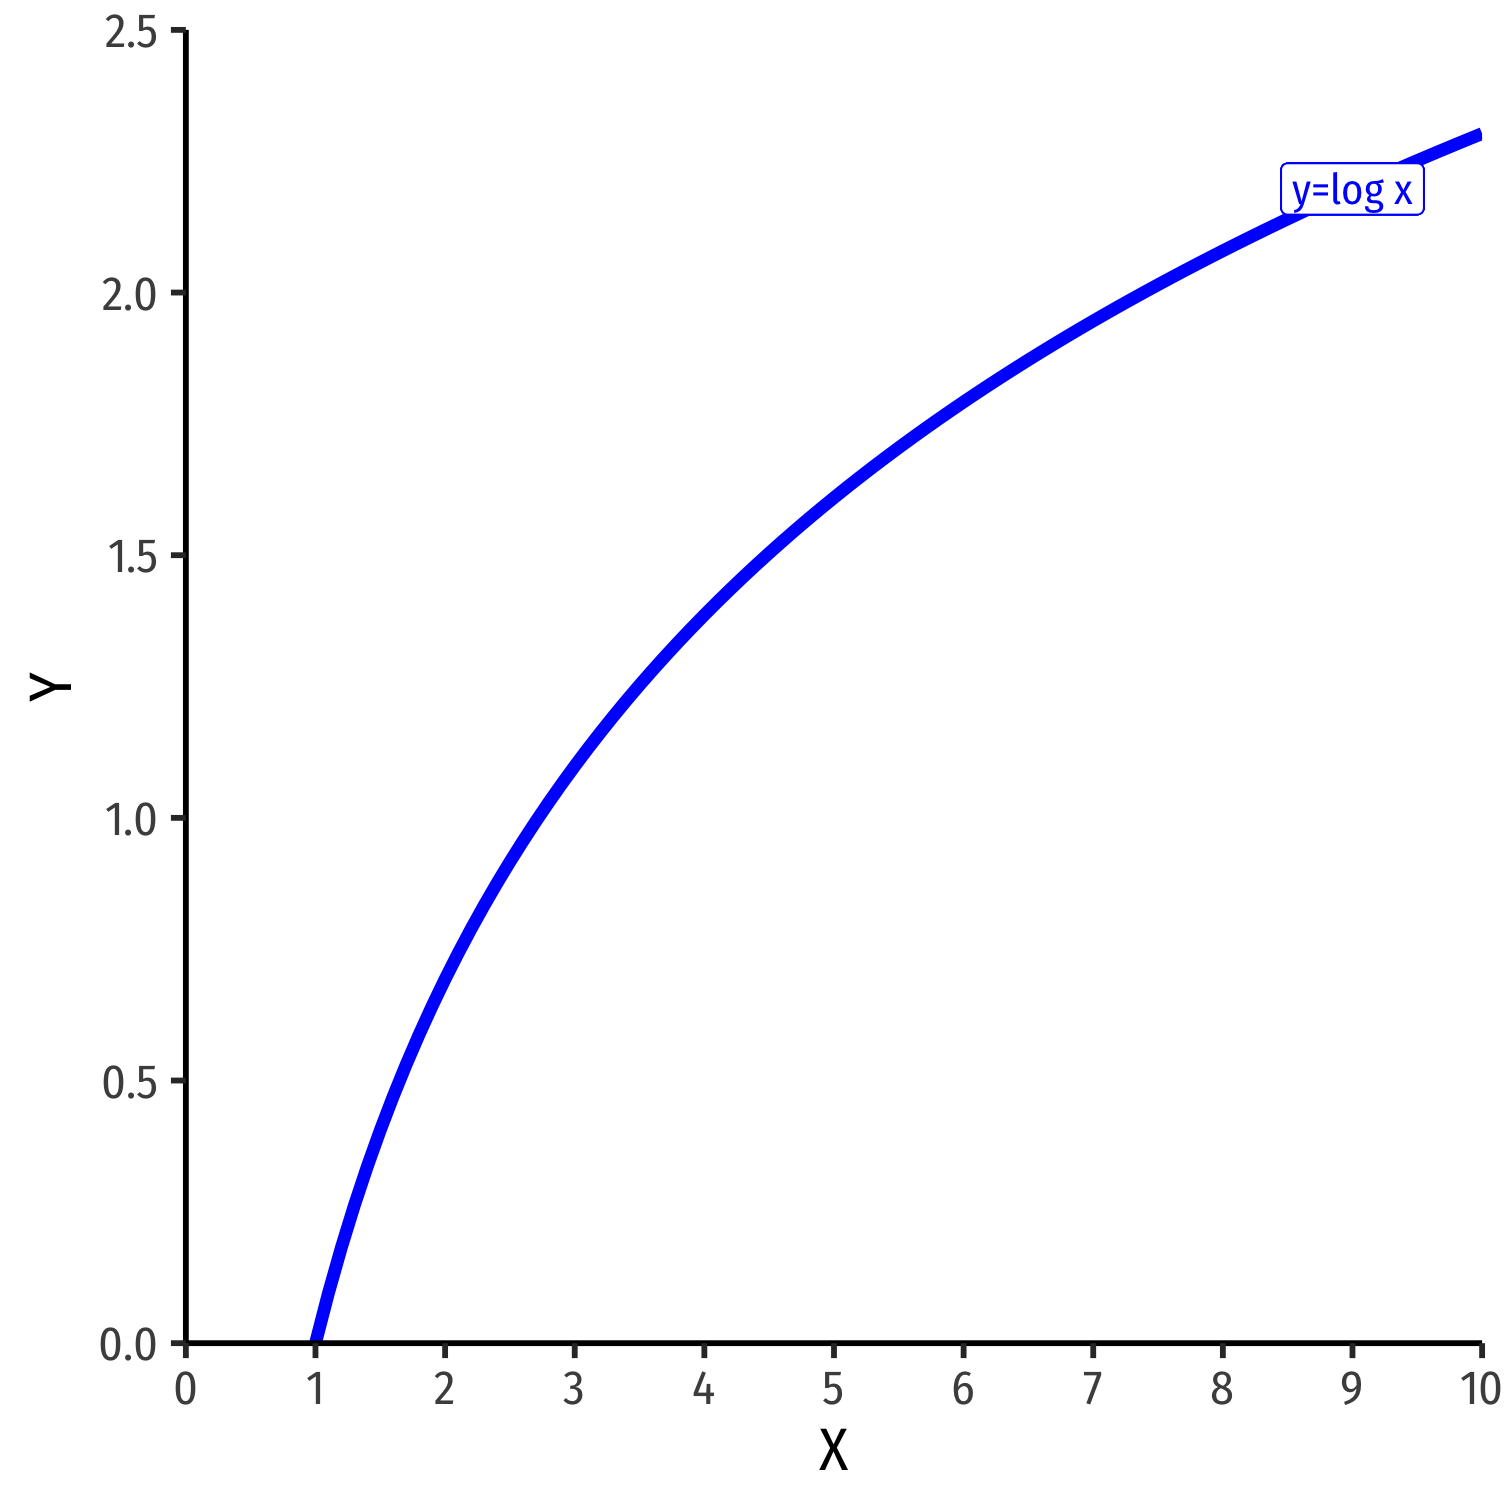
\includegraphics{01-problem-set-answers_files/figure-latex/unnamed-chunk-5-1.pdf}

\begin{Shaded}
\begin{Highlighting}[]
\KeywordTok{ggplot}\NormalTok{(}\DataTypeTok{data =}\NormalTok{ top_}\DecValTok{5}\NormalTok{_girls_}\DecValTok{2017}\NormalTok{)}\OperatorTok{+}
\StringTok{  }\KeywordTok{aes}\NormalTok{(}\DataTypeTok{x =} \KeywordTok{reorder}\NormalTok{(name, n), }\CommentTok{#note this reorders the x variable from small to large n}
      \DataTypeTok{y =}\NormalTok{ percent, }\CommentTok{# you can use prop if you didn't make a percent variable}
      \DataTypeTok{fill =}\NormalTok{ name)}\OperatorTok{+}\StringTok{ }\CommentTok{# optional color!}
\StringTok{  }\KeywordTok{geom_col}\NormalTok{()}\OperatorTok{+}
\StringTok{  }\CommentTok{# now I'm just making it pretty}
\StringTok{  }\KeywordTok{scale_y_continuous}\NormalTok{(}\DataTypeTok{labels=}\ControlFlowTok{function}\NormalTok{(x)}\KeywordTok{paste}\NormalTok{(x,}\StringTok{"%"}\NormalTok{,}\DataTypeTok{sep=}\StringTok{""}\NormalTok{))}\OperatorTok{+}\StringTok{ }\CommentTok{# optional, add percent signs}
\StringTok{      }\KeywordTok{labs}\NormalTok{(}\DataTypeTok{x =} \StringTok{"Name"}\NormalTok{,}
         \DataTypeTok{y =} \StringTok{"Percent of All Girls With Name"}\NormalTok{,}
         \DataTypeTok{title =} \StringTok{"Most Popular Girls Names Since 1880"}\NormalTok{,}
         \DataTypeTok{fill =} \StringTok{"Girl's Name"}\NormalTok{,}
         \DataTypeTok{caption =} \StringTok{"Source: SSA"}\NormalTok{)}\OperatorTok{+}
\StringTok{    }\KeywordTok{theme_classic}\NormalTok{(}\DataTypeTok{base_family =} \StringTok{"Fira Sans Condensed"}\NormalTok{, }\DataTypeTok{base_size=}\DecValTok{16}\NormalTok{)}\OperatorTok{+}
\StringTok{  }\KeywordTok{coord_flip}\NormalTok{()}\OperatorTok{+}\StringTok{ }\CommentTok{# rotate axes!}
\StringTok{  }\KeywordTok{theme}\NormalTok{(}\DataTypeTok{legend.position =} \StringTok{""}\NormalTok{) }\CommentTok{# hide legend}
\end{Highlighting}
\end{Shaded}

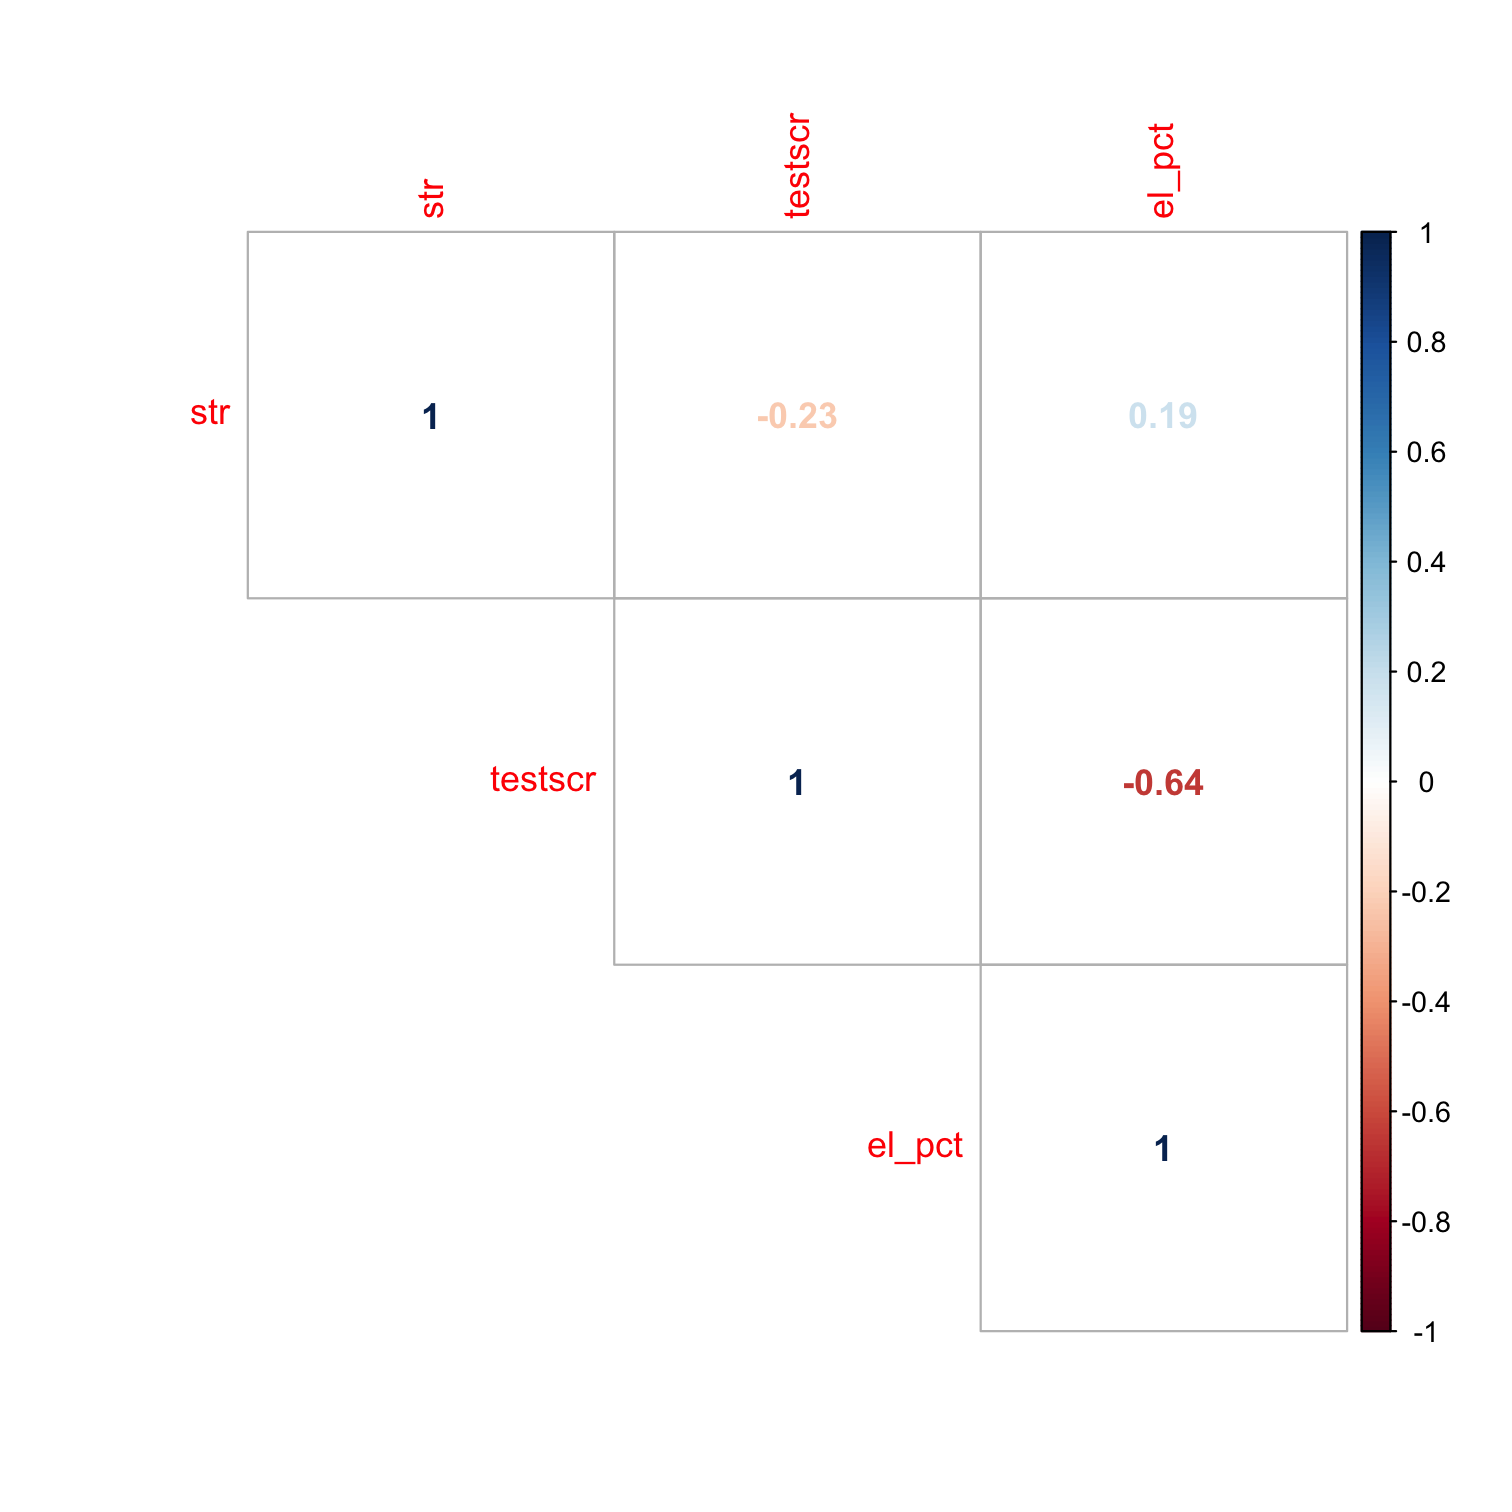
\includegraphics{01-problem-set-answers_files/figure-latex/unnamed-chunk-6-1.pdf}

\hypertarget{question-3}{%
\subsection{Question 3}\label{question-3}}

\textbf{Find your name.\footnote{If your name isn't in there :(, pick a
  random name.} \texttt{count} by \texttt{sex} how many babies since
1880 were named your name.\footnote{Hint: if you do this, you'll get the
  number of \emph{rows} (years) there are in the data. You want to add
  the number of babies in each row (\texttt{n}), so inside
  \texttt{count}, add \texttt{wt=n} to weight the count by \texttt{n}.}
Also add a variable for the percent of each sex.}

\begin{Shaded}
\begin{Highlighting}[]
\NormalTok{babynames }\OperatorTok
\StringTok{  }\KeywordTok{filter}\NormalTok{(name }\OperatorTok{==}\StringTok{ "Ryan"}\NormalTok{) }\OperatorTok
\StringTok{  }\KeywordTok{count}\NormalTok{(sex, }\DataTypeTok{wt=}\NormalTok{n) }\OperatorTok
\StringTok{  }\KeywordTok{mutate}\NormalTok{(}\DataTypeTok{percent =} \KeywordTok{round}\NormalTok{((n}\OperatorTok{/}\KeywordTok{sum}\NormalTok{(n)}\OperatorTok{*}\DecValTok{100}\NormalTok{),}\DecValTok{2}\NormalTok{))}
\end{Highlighting}
\end{Shaded}

\begin{verbatim}
## # A tibble: 2 x 3
##   sex        n percent
##   <chr>  <int>   <dbl>
## 1 F      22910    2.42
## 2 M     924877   97.6
\end{verbatim}

\hypertarget{question-4}{%
\subsection{Question 4}\label{question-4}}

\textbf{Make a line graph of the number of babies with your name over
time, \texttt{color}ed by \texttt{sex}.}

\begin{Shaded}
\begin{Highlighting}[]
\CommentTok{# note here I'm going to wrangle the data and then pipe it directly into ggplot}
\CommentTok{# you can wrangle the data and save it as a different tibble, then use THAT tibble}
\CommentTok{# for your (data = ...) command in ggplot}

\CommentTok{# first wrangle data}
\NormalTok{babynames }\OperatorTok
\StringTok{  }\KeywordTok{filter}\NormalTok{(name }\OperatorTok{==}\StringTok{ "Ryan"}\NormalTok{) }\OperatorTok

\StringTok{  }\CommentTok{# now we pipe into ggplot}
\StringTok{  }\KeywordTok{ggplot}\NormalTok{(}\DataTypeTok{data =}\NormalTok{ .)}\OperatorTok{+}\StringTok{ }\CommentTok{# the "." is a placeholder for the stuff above!}
\StringTok{  }\KeywordTok{aes}\NormalTok{(}\DataTypeTok{x =}\NormalTok{ year,}
      \DataTypeTok{y =}\NormalTok{ n,}
      \DataTypeTok{color =}\NormalTok{ sex)}\OperatorTok{+}
\StringTok{  }\KeywordTok{geom_line}\NormalTok{(}\DataTypeTok{size=}\DecValTok{1}\NormalTok{)}\OperatorTok{+}
\StringTok{  }\KeywordTok{labs}\NormalTok{(}\DataTypeTok{x =} \StringTok{"Year"}\NormalTok{,}
       \DataTypeTok{y =} \StringTok{"Number of Babies"}\NormalTok{,}
       \DataTypeTok{title =} \StringTok{"Popularity of Babies Named 'Ryan'"}\NormalTok{,}
       \DataTypeTok{color =} \StringTok{"Sex"}\NormalTok{,}
       \DataTypeTok{caption =} \StringTok{"Source: SSA"}\NormalTok{)}\OperatorTok{+}
\StringTok{    }\KeywordTok{theme_classic}\NormalTok{(}\DataTypeTok{base_family =} \StringTok{"Fira Sans Condensed"}\NormalTok{, }\DataTypeTok{base_size=}\DecValTok{16}\NormalTok{)}
\end{Highlighting}
\end{Shaded}

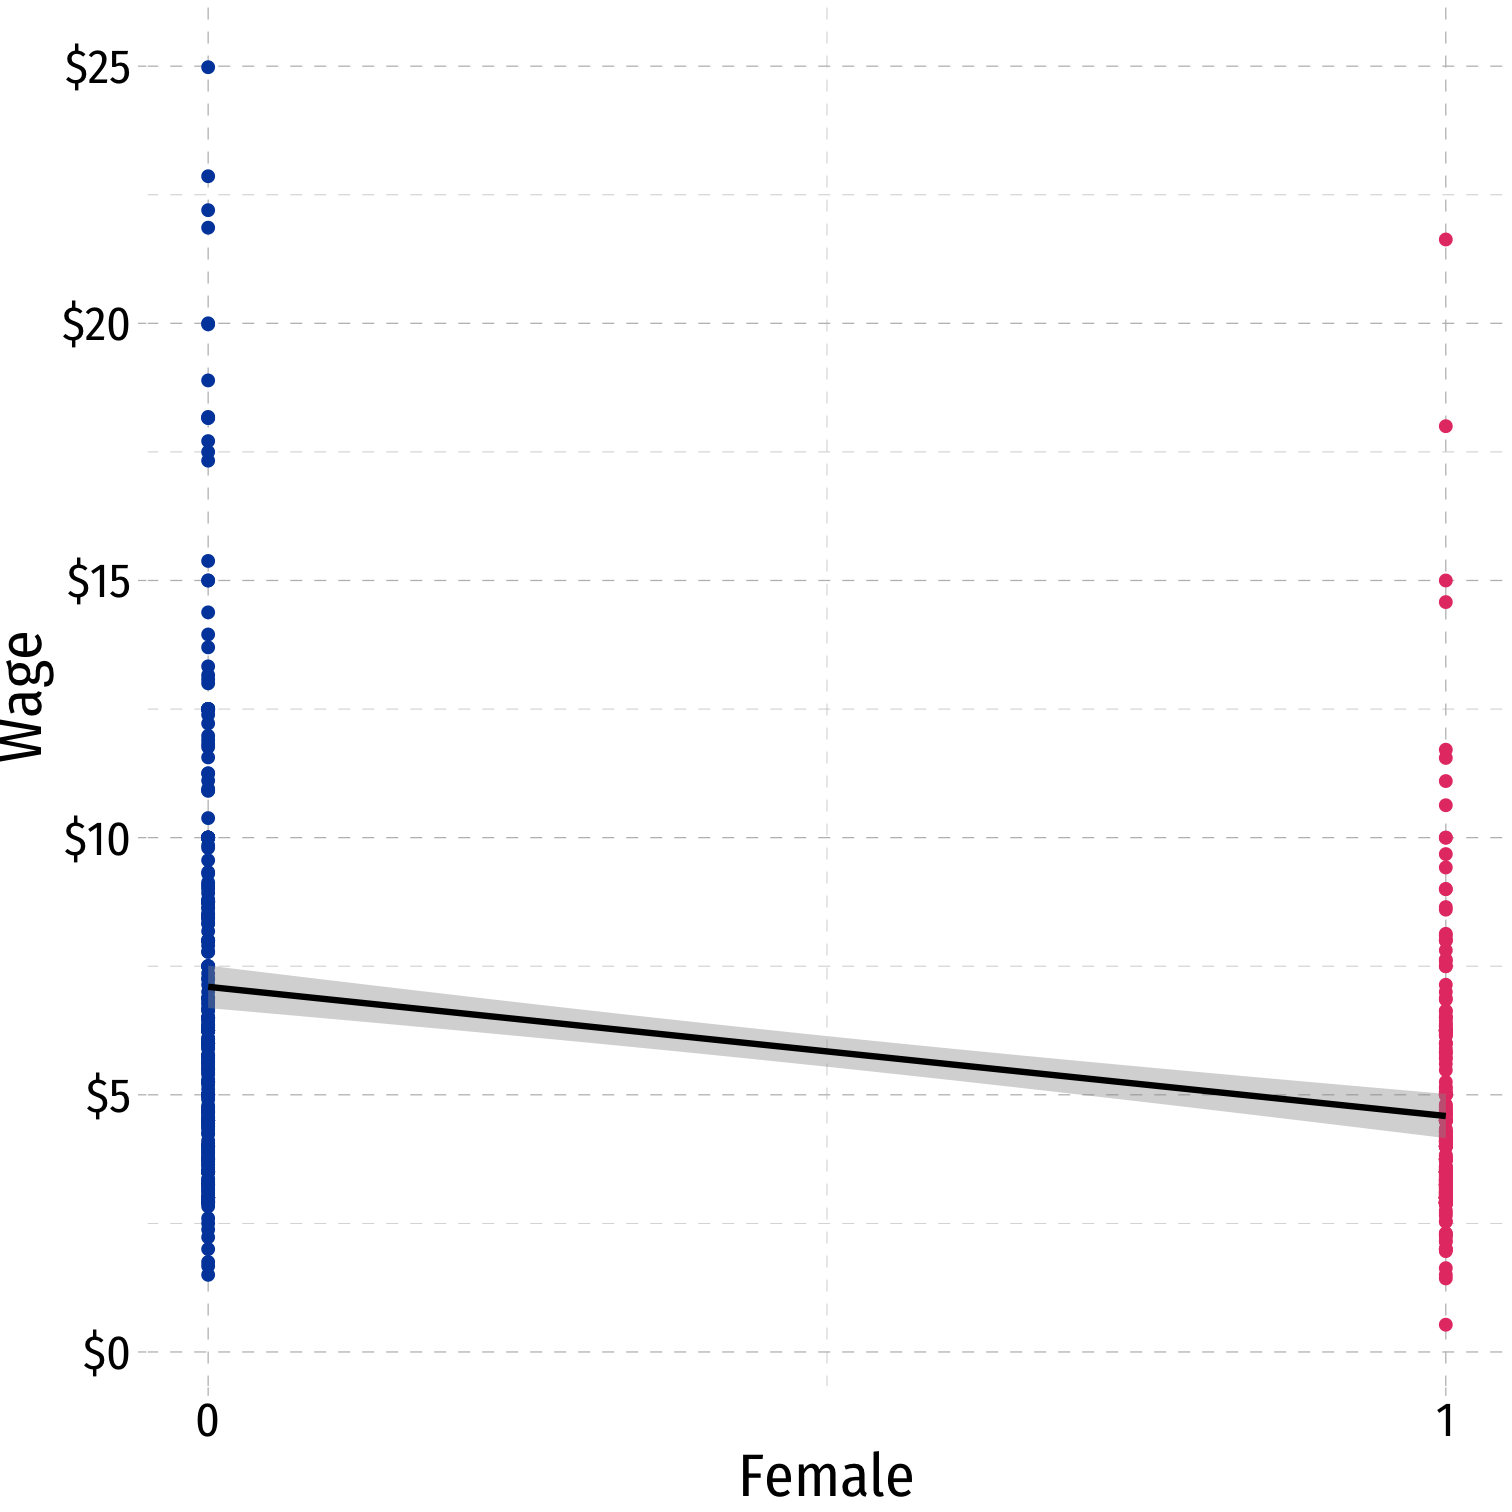
\includegraphics{01-problem-set-answers_files/figure-latex/unnamed-chunk-8-1.pdf}

\hypertarget{question-5}{%
\subsection{Question 5}\label{question-5}}

\hypertarget{part-a-1}{%
\subsubsection{Part A}\label{part-a-1}}

\textbf{Make a table of the most common name for boys by year between
1980-2017.\footnote{Hint: once you've got all the right conditions,
  you'll get a table with a lot of data. You only want to \texttt{slice}
  the \texttt{1}st row for each table.}}

\begin{Shaded}
\begin{Highlighting}[]
\NormalTok{babynames }\OperatorTok
\StringTok{  }\KeywordTok{group_by}\NormalTok{(year) }\OperatorTok\StringTok{ }\CommentTok{# we want one observation per year}
\StringTok{  }\KeywordTok{filter}\NormalTok{(sex }\OperatorTok{==}\StringTok{ "M"}\NormalTok{,}
\NormalTok{         year}\OperatorTok{>}\DecValTok{1979}\NormalTok{) }\OperatorTok\StringTok{ }\CommentTok{# or >==1980}
\StringTok{  }\KeywordTok{arrange}\NormalTok{(}\KeywordTok{desc}\NormalTok{(n))}\OperatorTok\StringTok{ }\CommentTok{# start with largest n first}
\StringTok{  }\KeywordTok{slice}\NormalTok{(}\DecValTok{1}\NormalTok{) }\CommentTok{# take first row only}
\end{Highlighting}
\end{Shaded}

\begin{verbatim}
## # A tibble: 38 x 5
## # Groups:   year [38]
##     year sex   name        n   prop
##    <dbl> <chr> <chr>   <int>  <dbl>
##  1  1980 M     Michael 68693 0.0370
##  2  1981 M     Michael 68765 0.0369
##  3  1982 M     Michael 68228 0.0362
##  4  1983 M     Michael 67995 0.0365
##  5  1984 M     Michael 67736 0.0361
##  6  1985 M     Michael 64906 0.0337
##  7  1986 M     Michael 64205 0.0334
##  8  1987 M     Michael 63647 0.0326
##  9  1988 M     Michael 64133 0.0320
## 10  1989 M     Michael 65382 0.0312
## # ... with 28 more rows
\end{verbatim}

\hypertarget{part-b-1}{%
\subsubsection{Part B}\label{part-b-1}}

\textbf{Now do the same for girls.}

\begin{Shaded}
\begin{Highlighting}[]
\NormalTok{babynames }\OperatorTok
\StringTok{  }\KeywordTok{group_by}\NormalTok{(year) }\OperatorTok\StringTok{ }\CommentTok{# we want one observation per year}
\StringTok{  }\KeywordTok{filter}\NormalTok{(sex }\OperatorTok{==}\StringTok{ "F"}\NormalTok{,}
\NormalTok{         year}\OperatorTok{>}\DecValTok{1979}\NormalTok{) }\OperatorTok\StringTok{ }\CommentTok{# or >==1980}
\StringTok{  }\KeywordTok{arrange}\NormalTok{(}\KeywordTok{desc}\NormalTok{(n))}\OperatorTok\StringTok{ }\CommentTok{# start with largest n first}
\StringTok{  }\KeywordTok{slice}\NormalTok{(}\DecValTok{1}\NormalTok{) }\CommentTok{# take first row only}
\end{Highlighting}
\end{Shaded}

\begin{verbatim}
## # A tibble: 38 x 5
## # Groups:   year [38]
##     year sex   name         n   prop
##    <dbl> <chr> <chr>    <int>  <dbl>
##  1  1980 F     Jennifer 58376 0.0328
##  2  1981 F     Jennifer 57049 0.0319
##  3  1982 F     Jennifer 57115 0.0315
##  4  1983 F     Jennifer 54342 0.0304
##  5  1984 F     Jennifer 50561 0.0280
##  6  1985 F     Jessica  48346 0.0262
##  7  1986 F     Jessica  52674 0.0285
##  8  1987 F     Jessica  55991 0.0299
##  9  1988 F     Jessica  51538 0.0268
## 10  1989 F     Jessica  47885 0.0240
## # ... with 28 more rows
\end{verbatim}

\hypertarget{question-6}{%
\subsection{Question 6}\label{question-6}}

\textbf{Now let's graph the evolution of the most common names since
1880.}

\hypertarget{part-a-2}{%
\subsubsection{Part A}\label{part-a-2}}

\textbf{First, find out what are the top 10 \emph{overall} most popular
names for boys and for girls. You may want to create two vectors, each
with these top 5 names.}

\begin{Shaded}
\begin{Highlighting}[]
\NormalTok{babynames }\OperatorTok
\StringTok{  }\KeywordTok{group_by}\NormalTok{(name) }\OperatorTok\StringTok{ }\CommentTok{# we want one row per name}
\StringTok{  }\KeywordTok{filter}\NormalTok{(sex}\OperatorTok{==}\StringTok{"M"}\NormalTok{) }\OperatorTok
\StringTok{  }\KeywordTok{summarize}\NormalTok{(}\DataTypeTok{total=}\KeywordTok{sum}\NormalTok{(n)) }\OperatorTok\StringTok{ }\CommentTok{# add upp all of the n's for all years for each name}
\StringTok{  }\KeywordTok{arrange}\NormalTok{(}\KeywordTok{desc}\NormalTok{(total)) }\OperatorTok\StringTok{ }\CommentTok{# list largest total first}
\StringTok{  }\KeywordTok{slice}\NormalTok{(}\DecValTok{1}\OperatorTok{:}\DecValTok{5}\NormalTok{) }
\end{Highlighting}
\end{Shaded}

\begin{verbatim}
## `summarise()` ungrouping output (override with `.groups` argument)
\end{verbatim}

\begin{verbatim}
## # A tibble: 5 x 2
##   name      total
##   <chr>     <int>
## 1 James   5150472
## 2 John    5115466
## 3 Robert  4814815
## 4 Michael 4350824
## 5 William 4102604
\end{verbatim}

\begin{Shaded}
\begin{Highlighting}[]
\CommentTok{# make a vector of the names (we'll need this for our graph below)}
\NormalTok{top_boys_names<-}\KeywordTok{c}\NormalTok{(}\StringTok{"James"}\NormalTok{, }\StringTok{"John"}\NormalTok{, }\StringTok{"Robert"}\NormalTok{, }\StringTok{"Michael"}\NormalTok{, }\StringTok{"William"}\NormalTok{)}

\CommentTok{# you could alternatively add a command, }
\CommentTok{# %>% pull(name) to the first chunk of code, }
\CommentTok{# and it would do the same thing, but we'd want to save it, }
\CommentTok{# for example:}

\NormalTok{babynames }\OperatorTok
\StringTok{  }\KeywordTok{group_by}\NormalTok{(name) }\OperatorTok\StringTok{ }\CommentTok{# we want one row per name}
\StringTok{  }\KeywordTok{filter}\NormalTok{(sex}\OperatorTok{==}\StringTok{"M"}\NormalTok{) }\OperatorTok
\StringTok{  }\KeywordTok{summarize}\NormalTok{(}\DataTypeTok{total=}\KeywordTok{sum}\NormalTok{(n)) }\OperatorTok\StringTok{ }\CommentTok{# add upp all of the n's for all years for each name}
\StringTok{  }\KeywordTok{arrange}\NormalTok{(}\KeywordTok{desc}\NormalTok{(total)) }\OperatorTok\StringTok{ }\CommentTok{# list largest total first}
\StringTok{  }\KeywordTok{slice}\NormalTok{(}\DecValTok{1}\OperatorTok{:}\DecValTok{5}\NormalTok{) }\OperatorTok
\StringTok{  }\KeywordTok{pull}\NormalTok{(name)}
\end{Highlighting}
\end{Shaded}

\begin{verbatim}
## `summarise()` ungrouping output (override with `.groups` argument)
\end{verbatim}

\begin{verbatim}
## [1] "James"   "John"    "Robert"  "Michael" "William"
\end{verbatim}

\begin{Shaded}
\begin{Highlighting}[]
\NormalTok{babynames }\OperatorTok
\StringTok{  }\KeywordTok{group_by}\NormalTok{(name) }\OperatorTok\StringTok{ }\CommentTok{# we want one row per name}
\StringTok{  }\KeywordTok{filter}\NormalTok{(sex}\OperatorTok{==}\StringTok{"F"}\NormalTok{) }\OperatorTok
\StringTok{  }\KeywordTok{summarize}\NormalTok{(}\DataTypeTok{total=}\KeywordTok{sum}\NormalTok{(n)) }\OperatorTok\StringTok{ }\CommentTok{# add upp all of the n's for all years for each name}
\StringTok{  }\KeywordTok{arrange}\NormalTok{(}\KeywordTok{desc}\NormalTok{(total)) }\OperatorTok\StringTok{ }\CommentTok{# list largest total first}
\StringTok{  }\KeywordTok{slice}\NormalTok{(}\DecValTok{1}\OperatorTok{:}\DecValTok{5}\NormalTok{)}
\end{Highlighting}
\end{Shaded}

\begin{verbatim}
## `summarise()` ungrouping output (override with `.groups` argument)
\end{verbatim}

\begin{verbatim}
## # A tibble: 5 x 2
##   name        total
##   <chr>       <int>
## 1 Mary      4123200
## 2 Elizabeth 1629679
## 3 Patricia  1571692
## 4 Jennifer  1466281
## 5 Linda     1452249
\end{verbatim}

\begin{Shaded}
\begin{Highlighting}[]
\CommentTok{# make a vector of the names (we'll need this for our graph below)}
\NormalTok{top_girls_names<-}\KeywordTok{c}\NormalTok{(}\StringTok{"Mary"}\NormalTok{, }\StringTok{"Elizabeth"}\NormalTok{, }\StringTok{"Patricia"}\NormalTok{, }\StringTok{"Jennifer"}\NormalTok{, }\StringTok{"Linda"}\NormalTok{)}
\end{Highlighting}
\end{Shaded}

\hypertarget{part-b-2}{%
\subsubsection{Part B}\label{part-b-2}}

\textbf{Now make two \texttt{line}graphs of these 5 names over time, one
for boys, and one for girls.}

\begin{Shaded}
\begin{Highlighting}[]
\NormalTok{babynames }\OperatorTok
\StringTok{  }\KeywordTok{group_by}\NormalTok{(year) }\OperatorTok
\StringTok{  }\KeywordTok{filter}\NormalTok{(sex }\OperatorTok{==}\StringTok{ "M"}\NormalTok{,}
\NormalTok{         name }\OperatorTok\StringTok{ }\NormalTok{top_boys_names) }\OperatorTok
\StringTok{  }\KeywordTok{ggplot}\NormalTok{(}\DataTypeTok{data =}\NormalTok{ .,}
         \KeywordTok{aes}\NormalTok{(}\DataTypeTok{x =}\NormalTok{ year,}
             \DataTypeTok{y =}\NormalTok{ prop,}
             \DataTypeTok{color =}\NormalTok{ name))}\OperatorTok{+}
\StringTok{  }\KeywordTok{geom_line}\NormalTok{()}\OperatorTok{+}
\StringTok{      }\KeywordTok{labs}\NormalTok{(}\DataTypeTok{x =} \StringTok{"Year"}\NormalTok{,}
         \DataTypeTok{y =} \StringTok{"Proportion of Babies with Name"}\NormalTok{,}
         \DataTypeTok{title =} \StringTok{"Most Popular Boys Names Since 1880"}\NormalTok{,}
         \DataTypeTok{color =} \StringTok{"Boy's Name"}\NormalTok{,}
         \DataTypeTok{caption =} \StringTok{"Source: SSA"}\NormalTok{)}\OperatorTok{+}
\StringTok{    }\KeywordTok{theme_classic}\NormalTok{(}\DataTypeTok{base_family =} \StringTok{"Fira Sans Condensed"}\NormalTok{, }\DataTypeTok{base_size=}\DecValTok{16}\NormalTok{)}
\end{Highlighting}
\end{Shaded}

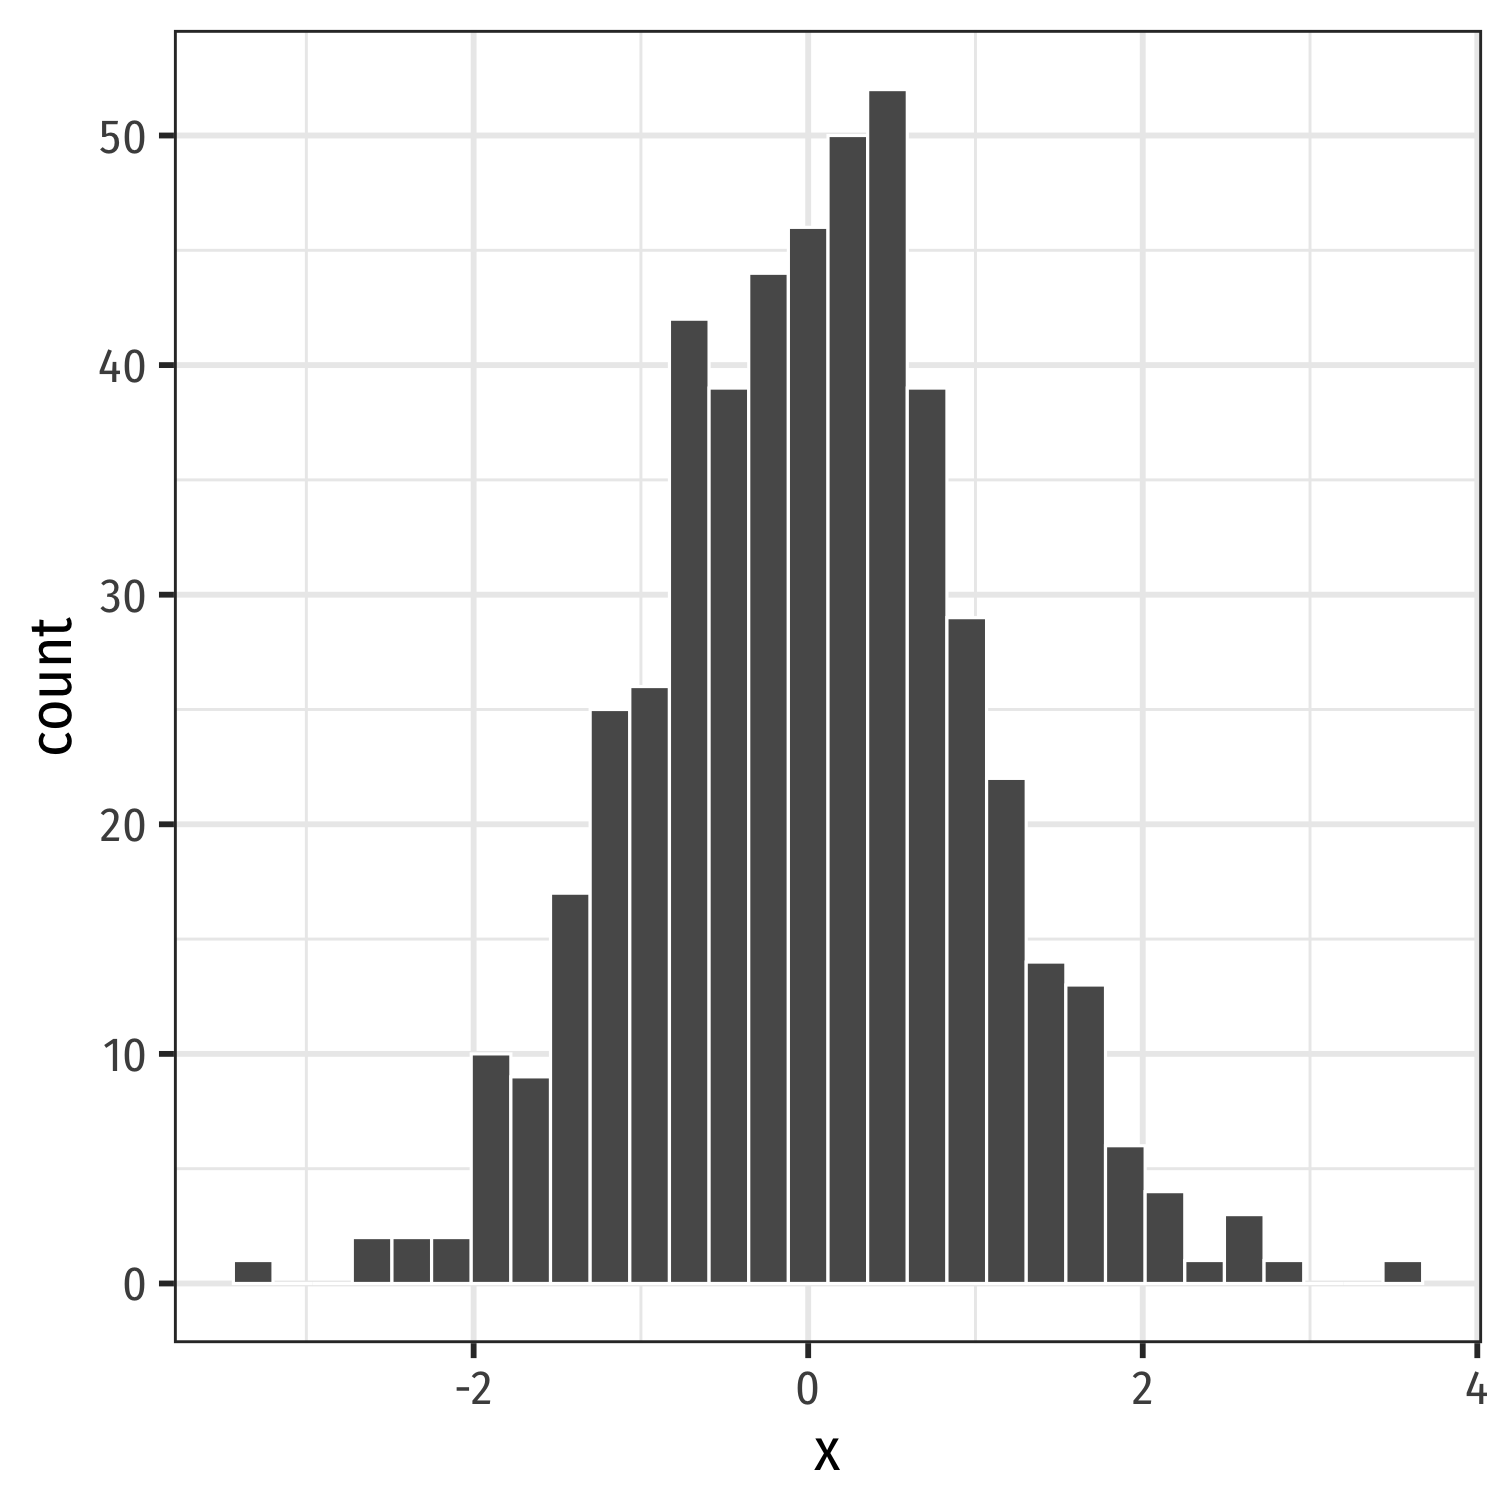
\includegraphics{01-problem-set-answers_files/figure-latex/unnamed-chunk-13-1.pdf}

\begin{Shaded}
\begin{Highlighting}[]
\NormalTok{babynames }\OperatorTok
\StringTok{  }\KeywordTok{group_by}\NormalTok{(year) }\OperatorTok
\StringTok{  }\KeywordTok{filter}\NormalTok{(sex }\OperatorTok{==}\StringTok{ "F"}\NormalTok{,}
\NormalTok{         name }\OperatorTok\StringTok{ }\NormalTok{top_girls_names) }\OperatorTok
\StringTok{  }\KeywordTok{ggplot}\NormalTok{(}\DataTypeTok{data =}\NormalTok{ .,}
         \KeywordTok{aes}\NormalTok{(}\DataTypeTok{x =}\NormalTok{ year,}
             \DataTypeTok{y =}\NormalTok{ prop,}
             \DataTypeTok{color =}\NormalTok{ name))}\OperatorTok{+}
\StringTok{  }\KeywordTok{geom_line}\NormalTok{()}\OperatorTok{+}
\StringTok{    }\KeywordTok{labs}\NormalTok{(}\DataTypeTok{x =} \StringTok{"Year"}\NormalTok{,}
         \DataTypeTok{y =} \StringTok{"Proportion of Babies with Name"}\NormalTok{,}
         \DataTypeTok{title =} \StringTok{"Most Popular Girls Names Since 1880"}\NormalTok{,}
         \DataTypeTok{color =} \StringTok{"Girl's Name"}\NormalTok{,}
         \DataTypeTok{caption =} \StringTok{"Source: SSA"}\NormalTok{)}\OperatorTok{+}
\StringTok{    }\KeywordTok{theme_classic}\NormalTok{(}\DataTypeTok{base_family =} \StringTok{"Fira Sans Condensed"}\NormalTok{, }\DataTypeTok{base_size=}\DecValTok{16}\NormalTok{)}
\end{Highlighting}
\end{Shaded}

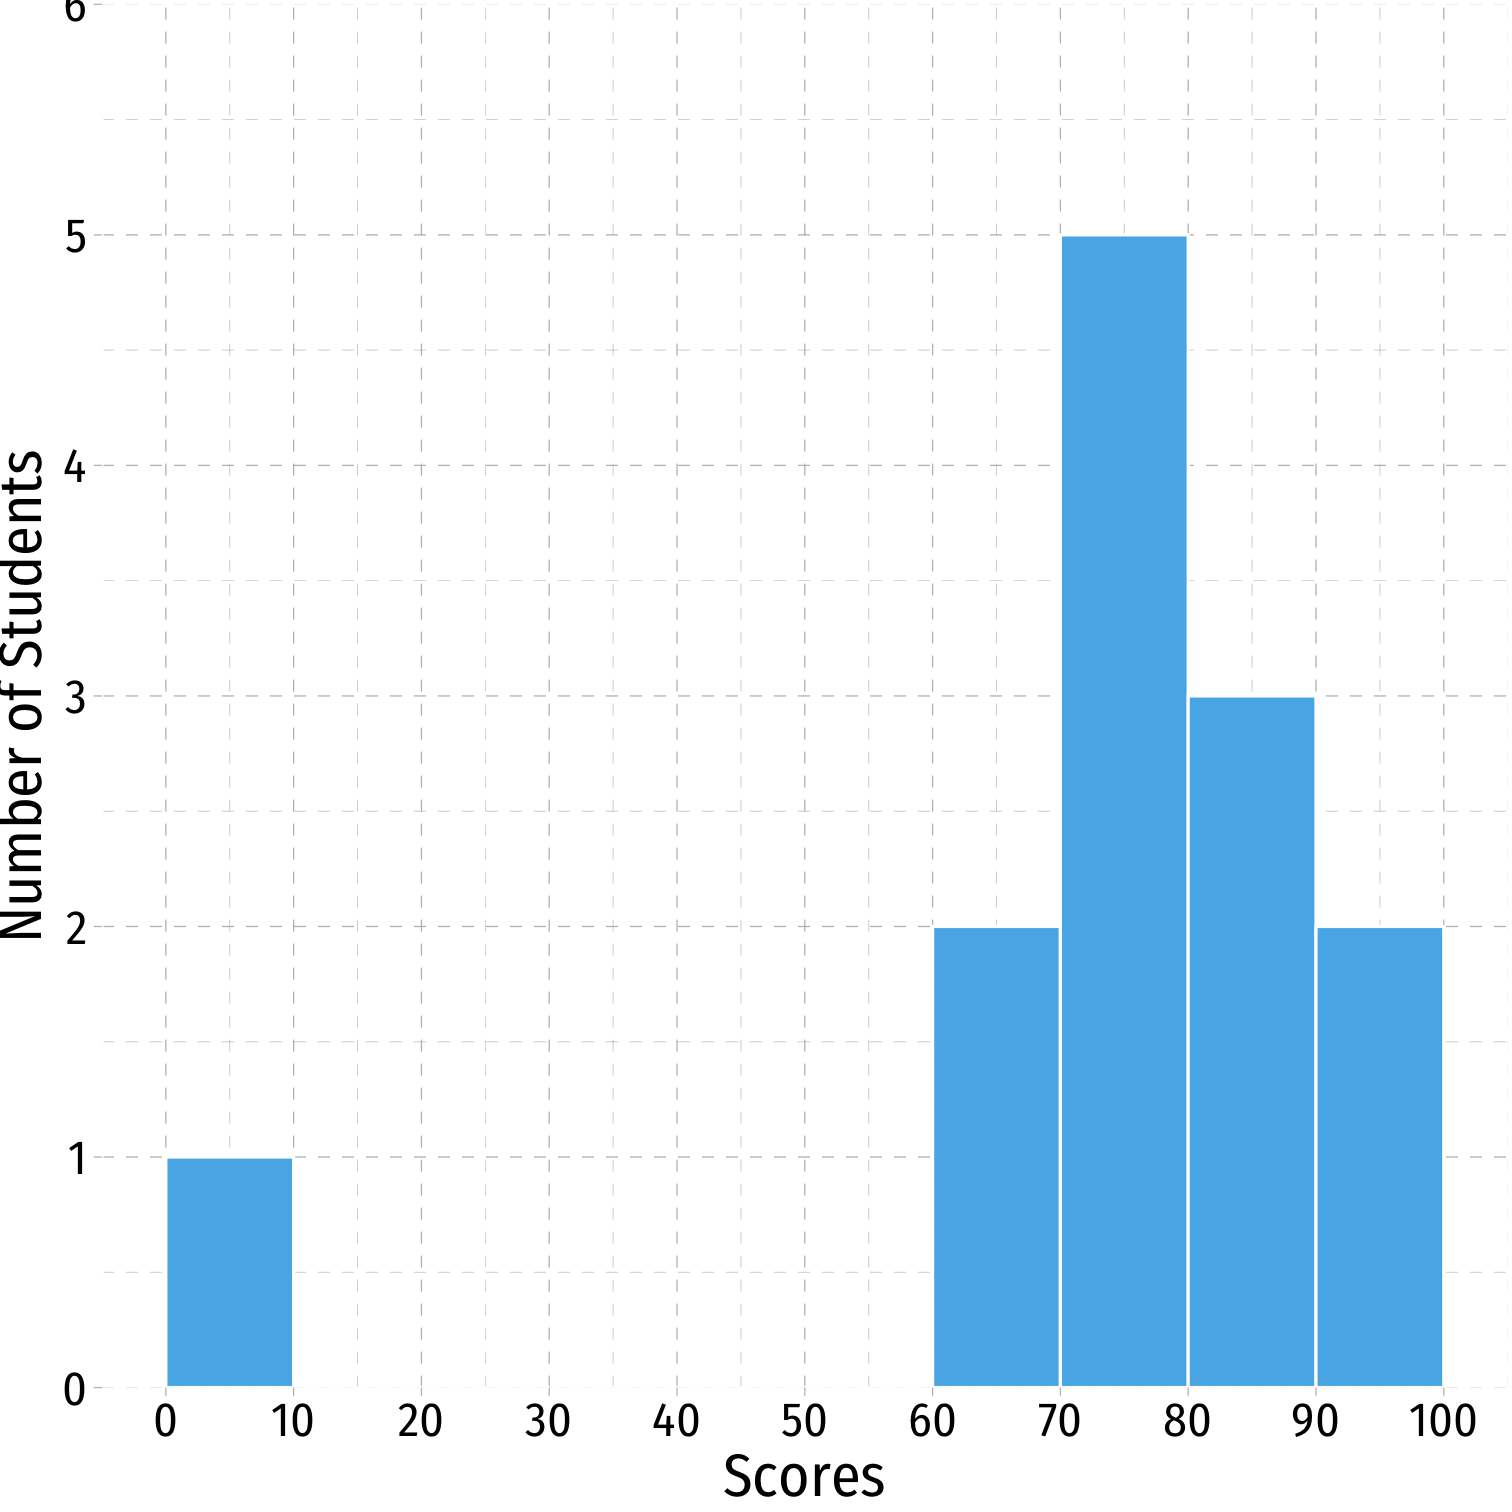
\includegraphics{01-problem-set-answers_files/figure-latex/unnamed-chunk-14-1.pdf}

\hypertarget{question-7}{%
\subsection{Question 7}\label{question-7}}

\textbf{\emph{Bonus (hard!)}: What are the 10 most common
``gender-neutral'' names?\footnote{This is hard to define. For our
  purposes, let's define this as names where between 48 and 52\% of the
  babies with the name are Male.}}

There's a lot to this, so I'll break this up step by step and show you
what happens at each major step.

We want to find the names where 48\% to 52\% of the babies with the name
are male, as I defined in the footnote. First let's \texttt{mutate} a
variable to figure out how many babies with a particular name are male.

To do this, we'll need to make a two variables to count the number of
\texttt{male}s and \texttt{female}s of each name each year. We'll use
the \texttt{ifelse()} function for each:

\begin{enumerate}
\def\labelenumi{\arabic{enumi}.}
\tightlist
\item
  Make a \texttt{male} variable where, for each name in each year, if
  \texttt{sex=="M"}, then count the number of males (\texttt{n}) that
  year, otherwise set it equal to \texttt{0}.
\item
  Make a \texttt{female} variable where, for each name in each year, if
  \texttt{sex=="F"}, then count the number of females (\texttt{n}) that
  year, otherwise set it equal to \texttt{0}.
\end{enumerate}

\begin{Shaded}
\begin{Highlighting}[]
\NormalTok{babynames }\OperatorTok
\StringTok{  }\KeywordTok{mutate}\NormalTok{(}\DataTypeTok{male =} \KeywordTok{ifelse}\NormalTok{(sex }\OperatorTok{==}\StringTok{ "M"}\NormalTok{, n, }\DecValTok{0}\NormalTok{),}
         \DataTypeTok{female =} \KeywordTok{ifelse}\NormalTok{(sex }\OperatorTok{==}\StringTok{ "F"}\NormalTok{, n, }\DecValTok{0}\NormalTok{))}
\end{Highlighting}
\end{Shaded}

\begin{verbatim}
## # A tibble: 1,924,665 x 7
##     year sex   name          n   prop  male female
##    <dbl> <chr> <chr>     <int>  <dbl> <dbl>  <dbl>
##  1  1880 F     Mary       7065 0.0724     0   7065
##  2  1880 F     Anna       2604 0.0267     0   2604
##  3  1880 F     Emma       2003 0.0205     0   2003
##  4  1880 F     Elizabeth  1939 0.0199     0   1939
##  5  1880 F     Minnie     1746 0.0179     0   1746
##  6  1880 F     Margaret   1578 0.0162     0   1578
##  7  1880 F     Ida        1472 0.0151     0   1472
##  8  1880 F     Alice      1414 0.0145     0   1414
##  9  1880 F     Bertha     1320 0.0135     0   1320
## 10  1880 F     Sarah      1288 0.0132     0   1288
## # ... with 1,924,655 more rows
\end{verbatim}

Now with this variable, we want to count the total number of males and
females with each name over the entire dataset. Let's first
\texttt{group\_by(name)} so we'll get one row for every name. We will
\texttt{summarize()} and take the \texttt{sum} of our \texttt{male} and
of our \texttt{female} variables.

\begin{Shaded}
\begin{Highlighting}[]
\NormalTok{babynames }\OperatorTok
\StringTok{  }\KeywordTok{mutate}\NormalTok{(}\DataTypeTok{male =} \KeywordTok{ifelse}\NormalTok{(sex }\OperatorTok{==}\StringTok{ "M"}\NormalTok{, n, }\DecValTok{0}\NormalTok{),}
         \DataTypeTok{female =} \KeywordTok{ifelse}\NormalTok{(sex }\OperatorTok{==}\StringTok{ "F"}\NormalTok{, n, }\DecValTok{0}\NormalTok{)) }\OperatorTok
\StringTok{  }\KeywordTok{group_by}\NormalTok{(name) }\OperatorTok
\StringTok{    }\KeywordTok{summarize}\NormalTok{(}\DataTypeTok{Male =} \KeywordTok{sum}\NormalTok{(male),}
              \DataTypeTok{Female =} \KeywordTok{sum}\NormalTok{(female))}
\end{Highlighting}
\end{Shaded}

\begin{verbatim}
## `summarise()` ungrouping output (override with `.groups` argument)
\end{verbatim}

\begin{verbatim}
## # A tibble: 97,310 x 3
##    name       Male Female
##    <chr>     <dbl>  <dbl>
##  1 Aaban       107      0
##  2 Aabha         0     35
##  3 Aabid        10      0
##  4 Aabir         5      0
##  5 Aabriella     0     32
##  6 Aada          0      5
##  7 Aadam       254      0
##  8 Aadan       130      0
##  9 Aadarsh     199      0
## 10 Aaden      4653      5
## # ... with 97,300 more rows
\end{verbatim}

Now, we want to figure out what \emph{fraction} of each name is Male or
Female. It doesn't matter which we do here, I'll do Male.
\texttt{mutate()} a new variable I'll call \texttt{perc\_male} for the
percent of the name being for Male babies. It takes the summed variables
we made before, and takes the fraction that are Male, multiplying by 100
to get percents (which isn't necessary, but is easy to read).

\begin{Shaded}
\begin{Highlighting}[]
\NormalTok{babynames }\OperatorTok
\StringTok{  }\KeywordTok{mutate}\NormalTok{(}\DataTypeTok{male =} \KeywordTok{ifelse}\NormalTok{(sex }\OperatorTok{==}\StringTok{ "M"}\NormalTok{, n, }\DecValTok{0}\NormalTok{),}
         \DataTypeTok{female =} \KeywordTok{ifelse}\NormalTok{(sex }\OperatorTok{==}\StringTok{ "F"}\NormalTok{, n, }\DecValTok{0}\NormalTok{)) }\OperatorTok
\StringTok{  }\KeywordTok{group_by}\NormalTok{(name) }\OperatorTok
\StringTok{    }\KeywordTok{summarize}\NormalTok{(}\DataTypeTok{Male =} \KeywordTok{sum}\NormalTok{(male),}
              \DataTypeTok{Female =} \KeywordTok{sum}\NormalTok{(female))}\OperatorTok
\StringTok{  }\KeywordTok{mutate}\NormalTok{(}\DataTypeTok{perc_male =}\NormalTok{ (Male}\OperatorTok{/}\NormalTok{(Male}\OperatorTok{+}\NormalTok{Female)}\OperatorTok{*}\DecValTok{100}\NormalTok{))}
\end{Highlighting}
\end{Shaded}

\begin{verbatim}
## `summarise()` ungrouping output (override with `.groups` argument)
\end{verbatim}

\begin{verbatim}
## # A tibble: 97,310 x 4
##    name       Male Female perc_male
##    <chr>     <dbl>  <dbl>     <dbl>
##  1 Aaban       107      0     100  
##  2 Aabha         0     35       0  
##  3 Aabid        10      0     100  
##  4 Aabir         5      0     100  
##  5 Aabriella     0     32       0  
##  6 Aada          0      5       0  
##  7 Aadam       254      0     100  
##  8 Aadan       130      0     100  
##  9 Aadarsh     199      0     100  
## 10 Aaden      4653      5      99.9
## # ... with 97,300 more rows
\end{verbatim}

Right now, it's still in alphabetical order. We want to arrange it by
\texttt{perc\_male}, and more importantly, we want \texttt{perc\_male}
to be between 48 and 52, so let's \texttt{filter} accordingly:

\begin{Shaded}
\begin{Highlighting}[]
\NormalTok{babynames }\OperatorTok
\StringTok{  }\KeywordTok{mutate}\NormalTok{(}\DataTypeTok{male =} \KeywordTok{ifelse}\NormalTok{(sex }\OperatorTok{==}\StringTok{ "M"}\NormalTok{, n, }\DecValTok{0}\NormalTok{),}
         \DataTypeTok{female =} \KeywordTok{ifelse}\NormalTok{(sex }\OperatorTok{==}\StringTok{ "F"}\NormalTok{, n, }\DecValTok{0}\NormalTok{)) }\OperatorTok
\StringTok{  }\KeywordTok{group_by}\NormalTok{(name) }\OperatorTok
\StringTok{    }\KeywordTok{summarize}\NormalTok{(}\DataTypeTok{Male =} \KeywordTok{sum}\NormalTok{(male),}
              \DataTypeTok{Female =} \KeywordTok{sum}\NormalTok{(female))}\OperatorTok
\StringTok{  }\KeywordTok{mutate}\NormalTok{(}\DataTypeTok{perc_male =}\NormalTok{ (Male}\OperatorTok{/}\NormalTok{(Male}\OperatorTok{+}\NormalTok{Female)}\OperatorTok{*}\DecValTok{100}\NormalTok{)) }\OperatorTok
\StringTok{  }\KeywordTok{arrange}\NormalTok{(perc_male) }\OperatorTok
\StringTok{  }\KeywordTok{filter}\NormalTok{(perc_male }\OperatorTok{>}\StringTok{ }\DecValTok{48}\NormalTok{,}
\NormalTok{         perc_male }\OperatorTok{<}\StringTok{ }\DecValTok{52}\NormalTok{)}
\end{Highlighting}
\end{Shaded}

\begin{verbatim}
## `summarise()` ungrouping output (override with `.groups` argument)
\end{verbatim}

\begin{verbatim}
## # A tibble: 266 x 4
##    name        Male Female perc_male
##    <chr>      <dbl>  <dbl>     <dbl>
##  1 Demetrice   1623   1754      48.1
##  2 Shenan        25     27      48.1
##  3 Yael        3162   3414      48.1
##  4 Harlo        164    177      48.1
##  5 Daylyn       202    218      48.1
##  6 Oluwatosin   139    150      48.1
##  7 Chaning       13     14      48.1
##  8 Kirin        351    378      48.1
##  9 Odera         13     14      48.1
## 10 Jireh        644    693      48.2
## # ... with 256 more rows
\end{verbatim}

This gives us a lot of names, all falling between 48\% and 52\% male.
But we want the most popular names that are in this range. So let's
finally \texttt{mutate} a new variable called \texttt{total} that simply
adds the number of \texttt{Male} and \texttt{Female} babies with a name.
Then let's \texttt{arrange} our results by \texttt{desc(total)} to get
the largest first, and then \texttt{slice(1:10)} to get the top 10 only.

\begin{Shaded}
\begin{Highlighting}[]
\NormalTok{babynames }\OperatorTok
\StringTok{  }\KeywordTok{mutate}\NormalTok{(}\DataTypeTok{male =} \KeywordTok{ifelse}\NormalTok{(sex }\OperatorTok{==}\StringTok{ "M"}\NormalTok{, n, }\DecValTok{0}\NormalTok{),}
         \DataTypeTok{female =} \KeywordTok{ifelse}\NormalTok{(sex }\OperatorTok{==}\StringTok{ "F"}\NormalTok{, n, }\DecValTok{0}\NormalTok{)) }\OperatorTok
\StringTok{  }\KeywordTok{group_by}\NormalTok{(name) }\OperatorTok
\StringTok{    }\KeywordTok{summarize}\NormalTok{(}\DataTypeTok{Male =} \KeywordTok{sum}\NormalTok{(male),}
              \DataTypeTok{Female =} \KeywordTok{sum}\NormalTok{(female))}\OperatorTok
\StringTok{  }\KeywordTok{mutate}\NormalTok{(}\DataTypeTok{perc_male =}\NormalTok{ (Male}\OperatorTok{/}\NormalTok{(Male}\OperatorTok{+}\NormalTok{Female)}\OperatorTok{*}\DecValTok{100}\NormalTok{)) }\OperatorTok
\StringTok{  }\KeywordTok{arrange}\NormalTok{(perc_male) }\OperatorTok
\StringTok{  }\KeywordTok{filter}\NormalTok{(perc_male }\OperatorTok{>}\StringTok{ }\DecValTok{48}\NormalTok{,}
\NormalTok{         perc_male }\OperatorTok{<}\StringTok{ }\DecValTok{52}\NormalTok{) }\OperatorTok
\StringTok{  }\KeywordTok{mutate}\NormalTok{(}\DataTypeTok{total =}\NormalTok{ Male}\OperatorTok{+}\NormalTok{Female) }\OperatorTok
\StringTok{  }\KeywordTok{arrange}\NormalTok{(}\KeywordTok{desc}\NormalTok{(total)) }\OperatorTok
\StringTok{  }\KeywordTok{slice}\NormalTok{(}\DecValTok{1}\OperatorTok{:}\DecValTok{10}\NormalTok{)}
\end{Highlighting}
\end{Shaded}

\begin{verbatim}
## `summarise()` ungrouping output (override with `.groups` argument)
\end{verbatim}

\begin{verbatim}
## # A tibble: 10 x 5
##    name      Male Female perc_male total
##    <chr>    <dbl>  <dbl>     <dbl> <dbl>
##  1 Kerry    49596  48534      50.5 98130
##  2 Robbie   20863  22264      48.4 43127
##  3 Justice  17080  15782      52.0 32862
##  4 Blair    14470  14195      50.5 28665
##  5 Kris     13982  13490      50.9 27472
##  6 Elisha   13330  13599      49.5 26929
##  7 Unknown   9307   9416      49.7 18723
##  8 Mckinley  9389   8955      51.2 18344
##  9 Baby      6078   5871      50.9 11949
## 10 Santana   4651   4952      48.4  9603
\end{verbatim}

\hypertarget{political-and-economic-freedom-around-the-world}{%
\section{Political and Economic Freedom Around the
World}\label{political-and-economic-freedom-around-the-world}}

\textbf{For the remaining questions, we'll look at the relationship
between Economic Freedom and Political Freedom in countries around the
world today. Our data for economic freedom comes from the
\href{https://www.fraserinstitute.org/economic-freedom/dataset?geozone=world\&year=2016\&page=dataset}{Fraser
Institute}, and our data for political freedom comes from
\href{https://freedomhouse.org/content/freedom-world-data-and-resources}{Freedom
House}.}

\hypertarget{question-8}{%
\subsection{Question 8}\label{question-8}}

\textbf{Download these two datasets that I've cleaned up a
bit:\footnote{If you want, try downloading them from the websites
  yourself!}}

\begin{itemize}
\tightlist
\item
  \href{http://metricsf19.classes.ryansafner.com/data/econfreedom.csv}{
  \texttt{econfreedom.csv}}
\item
  \href{http://metricsf19.classes.ryansafner.com/data/freedomhouse2018.csv}{
  \texttt{freedomhouse2018.csv}}
\end{itemize}

\textbf{Load them with
\texttt{df\textless{}-read\_csv("name\_of\_the\_file.csv")} and save one
as \texttt{econfreedom} and the other as \texttt{polfreedom}. Look at
each \texttt{tibble} you've created.}

I am creating this document for/from the website, so these are all
stored in a folder called \texttt{data}, one folder up from my current
folder, \texttt{homeworks}. To get there, I go up one folder
(\texttt{..}) and move to \texttt{data}, where these \texttt{csv} files
are stored.

I suggest you either keep the data in the same folder as your \texttt{R}
working directory (always check with \texttt{getwd()}), or create an R
Project and store the data files in that same folder.

\begin{Shaded}
\begin{Highlighting}[]
\CommentTok{# import data with read_csv from readr}

\CommentTok{# note these file paths will be different for you}
\NormalTok{polfreedom<-}\KeywordTok{read_csv}\NormalTok{(}\StringTok{"../data/freedomhouse2018.csv"}\NormalTok{)}
\end{Highlighting}
\end{Shaded}

\begin{verbatim}
## Parsed with column specification:
## cols(
##   .default = col_double(),
##   `Country/Territory` = col_character(),
##   Status = col_character()
## )
\end{verbatim}

\begin{verbatim}
## See spec(...) for full column specifications.
\end{verbatim}

\begin{Shaded}
\begin{Highlighting}[]
\NormalTok{econfreedom<-}\KeywordTok{read_csv}\NormalTok{(}\StringTok{"../data/econfreedom.csv"}\NormalTok{)}
\end{Highlighting}
\end{Shaded}

\begin{verbatim}
## Warning: Missing column names filled in: 'X1' [1]
\end{verbatim}

\begin{verbatim}
## Parsed with column specification:
## cols(
##   X1 = col_double(),
##   Country = col_character(),
##   ISO = col_character(),
##   ef = col_double(),
##   gdp = col_double(),
##   continent = col_character()
## )
\end{verbatim}

\begin{Shaded}
\begin{Highlighting}[]
\CommentTok{# look at each dataframe}
\NormalTok{polfreedom}
\end{Highlighting}
\end{Shaded}

\begin{verbatim}
## # A tibble: 209 x 40
##    `Country/Territ~ Status `PR Rating` `CL Rating`    A1    A2    A3     A    B1
##    <chr>            <chr>        <dbl>       <dbl> <dbl> <dbl> <dbl> <dbl> <dbl>
##  1 Abkhazia         PF               4           5     3     2     1     6     2
##  2 Afghanistan      NF               5           6     1     0     1     2     2
##  3 Albania          PF               3           3     3     3     2     8     3
##  4 Algeria          NF               6           5     1     1     1     3     1
##  5 Andorra          F                1           1     4     4     4    12     4
##  6 Angola           NF               6           6     0     2     1     3     2
##  7 Antigua and Bar~ F                2           2     4     4     4    12     3
##  8 Argentina        F                2           2     4     4     3    11     4
##  9 Armenia          PF               5           4     1     1     2     4     2
## 10 Australia        F                1           1     4     4     4    12     4
## # ... with 199 more rows, and 31 more variables: B2 <dbl>, B3 <dbl>, B4 <dbl>,
## #   B <dbl>, C1 <dbl>, C2 <dbl>, C3 <dbl>, C <dbl>, `Add Q` <dbl>, PR <dbl>,
## #   D1 <dbl>, D2 <dbl>, D3 <dbl>, D4 <dbl>, D <dbl>, E1 <dbl>, E2 <dbl>,
## #   E3 <dbl>, E <dbl>, F1 <dbl>, F2 <dbl>, F3 <dbl>, F4 <dbl>, F <dbl>,
## #   G1 <dbl>, G2 <dbl>, G3 <dbl>, G4 <dbl>, G <dbl>, CL <dbl>, Total <dbl>
\end{verbatim}

\begin{Shaded}
\begin{Highlighting}[]
\NormalTok{econfreedom}
\end{Highlighting}
\end{Shaded}

\begin{verbatim}
## # A tibble: 112 x 6
##       X1 Country    ISO      ef    gdp continent
##    <dbl> <chr>      <chr> <dbl>  <dbl> <chr>    
##  1     1 Albania    ALB    7.4   4543. Europe   
##  2     2 Algeria    DZA    5.15  4784. Africa   
##  3     3 Angola     AGO    5.08  4153. Africa   
##  4     4 Argentina  ARG    4.81 10502. Americas 
##  5     5 Australia  AUS    7.93 54688. Oceania  
##  6     6 Austria    AUT    7.56 47604. Europe   
##  7     7 Bahrain    BHR    7.6  22348. Asia     
##  8     8 Bangladesh BGD    6.35   973. Asia     
##  9     9 Belgium    BEL    7.51 45181. Europe   
## 10    10 Benin      BEN    6.22   805. Africa   
## # ... with 102 more rows
\end{verbatim}

\hypertarget{question-9}{%
\subsection{Question 9}\label{question-9}}

\textbf{The \texttt{polfreedom} dataset is still a bit messy. Let's
overwrite it (or assign to something like \texttt{polfreedom2}) and
select \texttt{Country/Territory} and \texttt{Total} (total freedom
score) and rename \texttt{Country.Territory} to \texttt{Country}.}

\begin{Shaded}
\begin{Highlighting}[]
\NormalTok{polfreedom<-polfreedom }\OperatorTok
\StringTok{  }\KeywordTok{select}\NormalTok{(}\StringTok{`}\DataTypeTok{Country/Territory}\StringTok{`}\NormalTok{, Total) }\OperatorTok
\StringTok{  }\KeywordTok{rename}\NormalTok{(}\DataTypeTok{Country=}\StringTok{`}\DataTypeTok{Country/Territory}\StringTok{`}\NormalTok{)}
\end{Highlighting}
\end{Shaded}

\hypertarget{question-10}{%
\subsection{Question 10}\label{question-10}}

\textbf{Now we can try to merge these two datasets into one. Since they
both have \texttt{Country} as a variable, we can merge these tibbles
using
\texttt{left\_join(econfreedom,\ polfreedom,\ by="Country")}\footnote{Note,
  if you saved as something else in question 9., use that instead of
  \texttt{polfreedom}!} and save this as a new tibble (something like
\texttt{freedom}).}

This one is a bit advanced to explain (but see the last few slides of
1.5 for more), so just copy what I gave you!

\begin{Shaded}
\begin{Highlighting}[]
\NormalTok{freedom<-}\KeywordTok{left_join}\NormalTok{(econfreedom, polfreedom, }\DataTypeTok{by=}\StringTok{"Country"}\NormalTok{)}
\end{Highlighting}
\end{Shaded}

\hypertarget{question-11}{%
\subsection{Question 11}\label{question-11}}

\textbf{Now make a scatterplot of Political Freedom
(\texttt{total})\footnote{Feel free to \texttt{rename} these!} as
\texttt{y} on Economic Freedom (\texttt{ef}) as \texttt{x} and
\texttt{color} by \texttt{continent}.}

\begin{verbatim}
## Warning: Removed 1 rows containing missing values (geom_point).
\end{verbatim}

\includegraphics[width=0.9\linewidth]{01-problem-set-answers_files/figure-latex/plot1-1}

\hypertarget{question-12}{%
\subsection{Question 12}\label{question-12}}

\textbf{Let's do this again, but highlight some key countries. Pick
three countries, and make a new tibble from \texttt{freedom} that is
only the observations of those countries. Additionally, \emph{install}
and \emph{load} a packaged called \texttt{ggrepel}\footnote{This
  automatically adjusts labels so they don't cover points on a plot!}
Next, redo your plot from question 11, but now add a layer:
\texttt{geom\_label\_repel} and set its \texttt{data} to your
three-country tibble, use same \texttt{aes}thetics as your overall plot,
but be sure to add \texttt{label\ =\ ISO}, to use the ISO country code
to label.\footnote{You might also want to set a low \texttt{alpha} level
  to make sure the labels don't obscure other points!}}

\begin{Shaded}
\begin{Highlighting}[]
\CommentTok{# install.packages("ggrepel") install for first use }
\KeywordTok{library}\NormalTok{(ggrepel) }\CommentTok{# load }

\NormalTok{interest<-}\KeywordTok{filter}\NormalTok{(freedom, ISO }\OperatorTok\StringTok{ }\KeywordTok{c}\NormalTok{(}\StringTok{"CHN"}\NormalTok{, }\StringTok{"NOR"}\NormalTok{, }\StringTok{"USA"}\NormalTok{))}

\KeywordTok{ggplot}\NormalTok{(}\DataTypeTok{data=}\NormalTok{freedom, }\KeywordTok{aes}\NormalTok{(}\DataTypeTok{x=}\NormalTok{ef,}\DataTypeTok{y=}\NormalTok{Total))}\OperatorTok{+}
\StringTok{  }\KeywordTok{geom_point}\NormalTok{(}\KeywordTok{aes}\NormalTok{(}\DataTypeTok{color=}\NormalTok{continent))}\OperatorTok{+}
\StringTok{  }\KeywordTok{geom_label_repel}\NormalTok{(}\DataTypeTok{data=}\NormalTok{interest, }\KeywordTok{aes}\NormalTok{(ef, Total, }\DataTypeTok{label=}\NormalTok{ISO,}\DataTypeTok{color=}\NormalTok{continent),}\DataTypeTok{alpha=}\FloatTok{0.6}\NormalTok{)}\OperatorTok{+}
\StringTok{  }\KeywordTok{xlab}\NormalTok{(}\StringTok{"Economic Freedom Score"}\NormalTok{)}\OperatorTok{+}\KeywordTok{ylab}\NormalTok{(}\StringTok{"Political Freedom Score"}\NormalTok{)}\OperatorTok{+}\KeywordTok{theme_bw}\NormalTok{()}\OperatorTok{+}\KeywordTok{labs}\NormalTok{(}\DataTypeTok{caption=}\StringTok{"Sources: Frasier Institute, Freedom House"}\NormalTok{)}\OperatorTok{+}
\StringTok{  }\KeywordTok{theme_classic}\NormalTok{(}\DataTypeTok{base_family =} \StringTok{"Fira Sans Condensed"}\NormalTok{, }\DataTypeTok{base_size=}\DecValTok{16}\NormalTok{)}
\end{Highlighting}
\end{Shaded}

\begin{verbatim}
## Warning: Removed 1 rows containing missing values (geom_point).
\end{verbatim}

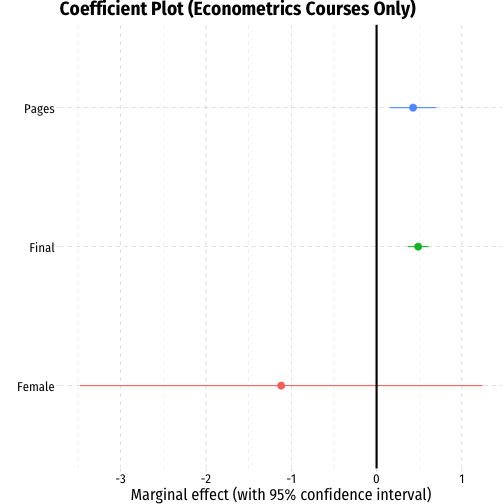
\includegraphics[width=468px]{01-problem-set-answers_files/figure-latex/unnamed-chunk-23-1}

\hypertarget{question-13}{%
\subsection{Question 13}\label{question-13}}

\textbf{Make another plot similar to 12, except this time use GDP per
Capita (\texttt{gdp}) as \texttt{y}. Feel free to try to put a
regression line with \texttt{geom\_smooth()}!}\footnote{If you do, be
  sure to set its data to the full \texttt{freedom}, not just your three
  countries!}. \textbf{Those of you in my Development course, you just
made my graphs from
\href{https://devf19.classes.ryansafner.com/slides/02-slides\#23}{Lesson
2}!}

\begin{Shaded}
\begin{Highlighting}[]
\KeywordTok{ggplot}\NormalTok{(}\DataTypeTok{data=}\NormalTok{freedom, }\KeywordTok{aes}\NormalTok{(}\DataTypeTok{x=}\NormalTok{ef,}\DataTypeTok{y=}\NormalTok{gdp))}\OperatorTok{+}
\StringTok{  }\KeywordTok{geom_point}\NormalTok{(}\KeywordTok{aes}\NormalTok{(}\DataTypeTok{color=}\NormalTok{continent))}\OperatorTok{+}
\StringTok{  }\KeywordTok{geom_smooth}\NormalTok{(}\DataTypeTok{data=}\NormalTok{freedom)}\OperatorTok{+}
\StringTok{  }\KeywordTok{geom_label_repel}\NormalTok{(}\DataTypeTok{data=}\NormalTok{interest, }\KeywordTok{aes}\NormalTok{(ef, Total, }\DataTypeTok{label=}\NormalTok{ISO,}\DataTypeTok{color=}\NormalTok{continent),}\DataTypeTok{alpha=}\FloatTok{0.6}\NormalTok{)}\OperatorTok{+}
\StringTok{  }\KeywordTok{xlab}\NormalTok{(}\StringTok{"Economic Freedom Score"}\NormalTok{)}\OperatorTok{+}\KeywordTok{ylab}\NormalTok{(}\StringTok{"Political Freedom Score"}\NormalTok{)}\OperatorTok{+}\KeywordTok{theme_bw}\NormalTok{()}\OperatorTok{+}\KeywordTok{labs}\NormalTok{(}\DataTypeTok{caption=}\StringTok{"Sources: Frasier Institute, Freedom House"}\NormalTok{)}\OperatorTok{+}
\StringTok{  }\KeywordTok{theme_classic}\NormalTok{(}\DataTypeTok{base_family =} \StringTok{"Fira Sans Condensed"}\NormalTok{, }\DataTypeTok{base_size=}\DecValTok{16}\NormalTok{)}
\end{Highlighting}
\end{Shaded}

\begin{verbatim}
## `geom_smooth()` using method = 'loess' and formula 'y ~ x'
\end{verbatim}

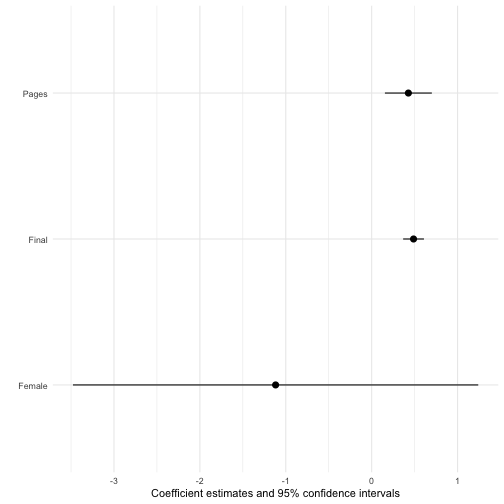
\includegraphics[width=468px]{01-problem-set-answers_files/figure-latex/unnamed-chunk-24-1}

\end{document}
